%%%%%%%%%%%%%%%%%%%%%%%%%%%%%%%%%%%%%%%%%%%%%%%%%%%%%%%%%%%%%%%%%%%%%%%%%%%%%%%%
%%  Sample document for preparing papers to  "Avtomatika i Telemekhanika"
%%  charset=utf-8
%%%%%%%%%%%%%%%%%%%%%%%%%%%%%%%%%%%%%%%%%%%%%%%%%%%%%%%%%%%%%%%%%%%%%%%%%%%%%%%%

\documentclass[12pt]{a&t}
\usepackage[all,cmtip]{xy}
\usepackage{graphicx}
\usepackage{tabularx}
\usepackage{algorithmic}
\usepackage{algorithm}
\usepackage{subcaption}

\begin{document}  %%%!!!

\year{2022}
\title{ГРАДИЕНТНЫЕ МЕТОДЫ ОПТИМИЗАЦИИ МЕТАПАРАМЕТРОВ В ЗАДАЧЕ ДИСТИЛЛЯЦИИ ЗНАНИЙ}

\thanks{Работа выполнена при поддержке Научной академической стипендии имени К. В. Рудакова}
% (грант \mbox{№\,\dots}).}

\authors{М.~ГОРПИНИЧ\\
(Московский физико-технический институт (государственный университет)),\\
О.Ю.~БАХТЕЕВ, канд.~физ.-мат.~наук\\
(Вычислительный центр имени А.А. Дородницына Федерального исследовательского центра
«Информатика и управление» Российской академии наук),\\
В.В.~СТРИЖОВ, д-р~физ.-мат.~наук\\
(Вычислительный центр имени А.А. Дородницына Федерального исследовательского центра
«Информатика и управление» Российской академии наук)}

\maketitle

\begin{abstract}
В работе исследуется задача дистилляции моделей глубокого обучения. Дистилляция знаний --- это задача оптимизации метапараметров, в которой происходит перенос информации модели более сложной структуры, называемой моделью-учителем, в модель более простой структуры, называемой моделью-учеником. В работе предлагается обобщение задачи дистилляции на случай оптимизации метапараметров градиентными методами. Метапараметрами являются параметры оптимизационной задачи дистилляции. В качестве функции потерь для такой задачи выступает сумма слагаемого классификации и кросс-энтропии между ответами модели-ученика и модели-учителя. Назначение оптимальных метапараметров в функции потерь дистилляции является вычислительно сложной задачей. Исследуются свойства оптимизационной задачи с целью предсказания траектории обновления метапараметров. Проводится анализ траектории градиентной оптимизации метапараметров и предсказывается их значение с помощью линейных функций. Предложенный подход проиллюстрирован с помощью вычислительного эксперимента на выборках CIFAR-10 и Fashion-MNIST, а также на синтетических данных. 
\end{abstract}

\textbf{Ключевые слова:} Машинное обучение,  Дистилляция знаний, Оптимизация метапараметров, Градиентная оптимизация, Назначение метапараметров.


\section{Введение}

В работе рассматривается задача дистилляции моделей глубокого обучения. Оптимизация модели глубокого обучения является вычислительно сложной задачей~\cite{rasley2020deepspeed}. В работе исследуется частный случай задачи оптимизации, называемый дистилляцией знаний. Он позволяет использовать одновременно обучающую выборку и информацию, содержащуюся в предобученных моделях. \textit{Дистилляцией знаний} \cite{journals/corr/HintonVD15} назовем задачу оптимизации параметров модели, в которой учитывается не только информация, содержащаяся в исходной выборке, но также и  информация, содержащаяся в \textit{модели-учителе}. Модель-учитель имеет высокую сложность. В ней содержится информация о выборке, а также о распределениях параметров модели, перенос которых будет осуществлен. Модель более простой структуры, называемая \textit{моделью-учеником}, оптимизируется путем переноса знаний модели-учителя.


Исследуется процедура оптимизации метапараметров в задаче дистилляции знаний.  \textit{Метапараметрами} являются параметры оптимизационной задачи. Корректное назначение метапараметров может существенно повлиять на качество итоговой модели~\cite{journals/corr/Pedregosa16}. В отличие от~\cite{journals/corr/Pedregosa16,journals/corr/MaclaurinDA15}, в данной работе учитывается различие между \textit{гиперпараметрами}, вероятностными параметрами априорного распределения~\cite{bishop2006pattern} и метапараметрами. Несмотря на количество методов оптимизации метапараметров и гиперпараметров, использующихся в глубоком обучении, таких как случайный поиск~\cite{bergstra2012random} или модели, основанные на использовании вероятностных моделей~\cite{bergstra2013making}, во многих подходах предлагается последовательно порождать случайное значение метапараметров и оценивать качество модели, обученной при данных значениях гиперпараметров. Данный подход может не подойти в случае обучения моделей, требующих значительных временных затрат для обучения. В Таблице~\ref{table:compl} содержатся сложности различных подходов к оптимизации метапараметров. Видно, что в случае, если оптимизация параметров занимает значительное время, подходы, требующие несколько запусков оптимизации являются неэффективными.

\begin{table}[]
\caption{Сложность различных методов оптимизации метапараметров и гиперпараметров. Здесь $|\mathbf{w}|$ является числом параметров модели, $|\boldsymbol{\lambda}|$ --- числом метапараметров, $r$ --- это количество запусков стохастических методов оптимизации, $s$ --- сложность порождения из вероятностных моделей.}
\centering
\begin{tabularx}{\textwidth}{X|X|X} \hline
\bf {Метод} & \bf {Тип метода оптимизации}  & \bf{Сложность}  \\ \hline \hline 
Случайный поиск~\cite{bergstra2012random} & Стохастический & $O(r\cdot|\mathbf{w}|)$      \\ \hline
Основанный на вероятностных моделях~\cite{bergstra2013making}  & Стохастический                                    & $O\left(r \cdot \left(|\mathbf{w}| + s\right)\right)$               \\ \hline
Жадный градиентный~\cite{journals/corr/LuketinaBR15}                    & Градиентный                                &$O(|\mathbf{w}|\cdot|\boldsymbol{\lambda}|)$    \\ \hline
Жадный градиентный с разностной аппроксимацией~\cite{liu2018darts} & Градиентный                                & $O(|\mathbf{w}| + |\boldsymbol{\lambda}|)$   \\ \hline
\end{tabularx}
\vspace{0.2cm}
\label{table:compl}

\end{table}

\begin{figure}[ht]
    % \vspace{-0.3 cm}
    \center{
    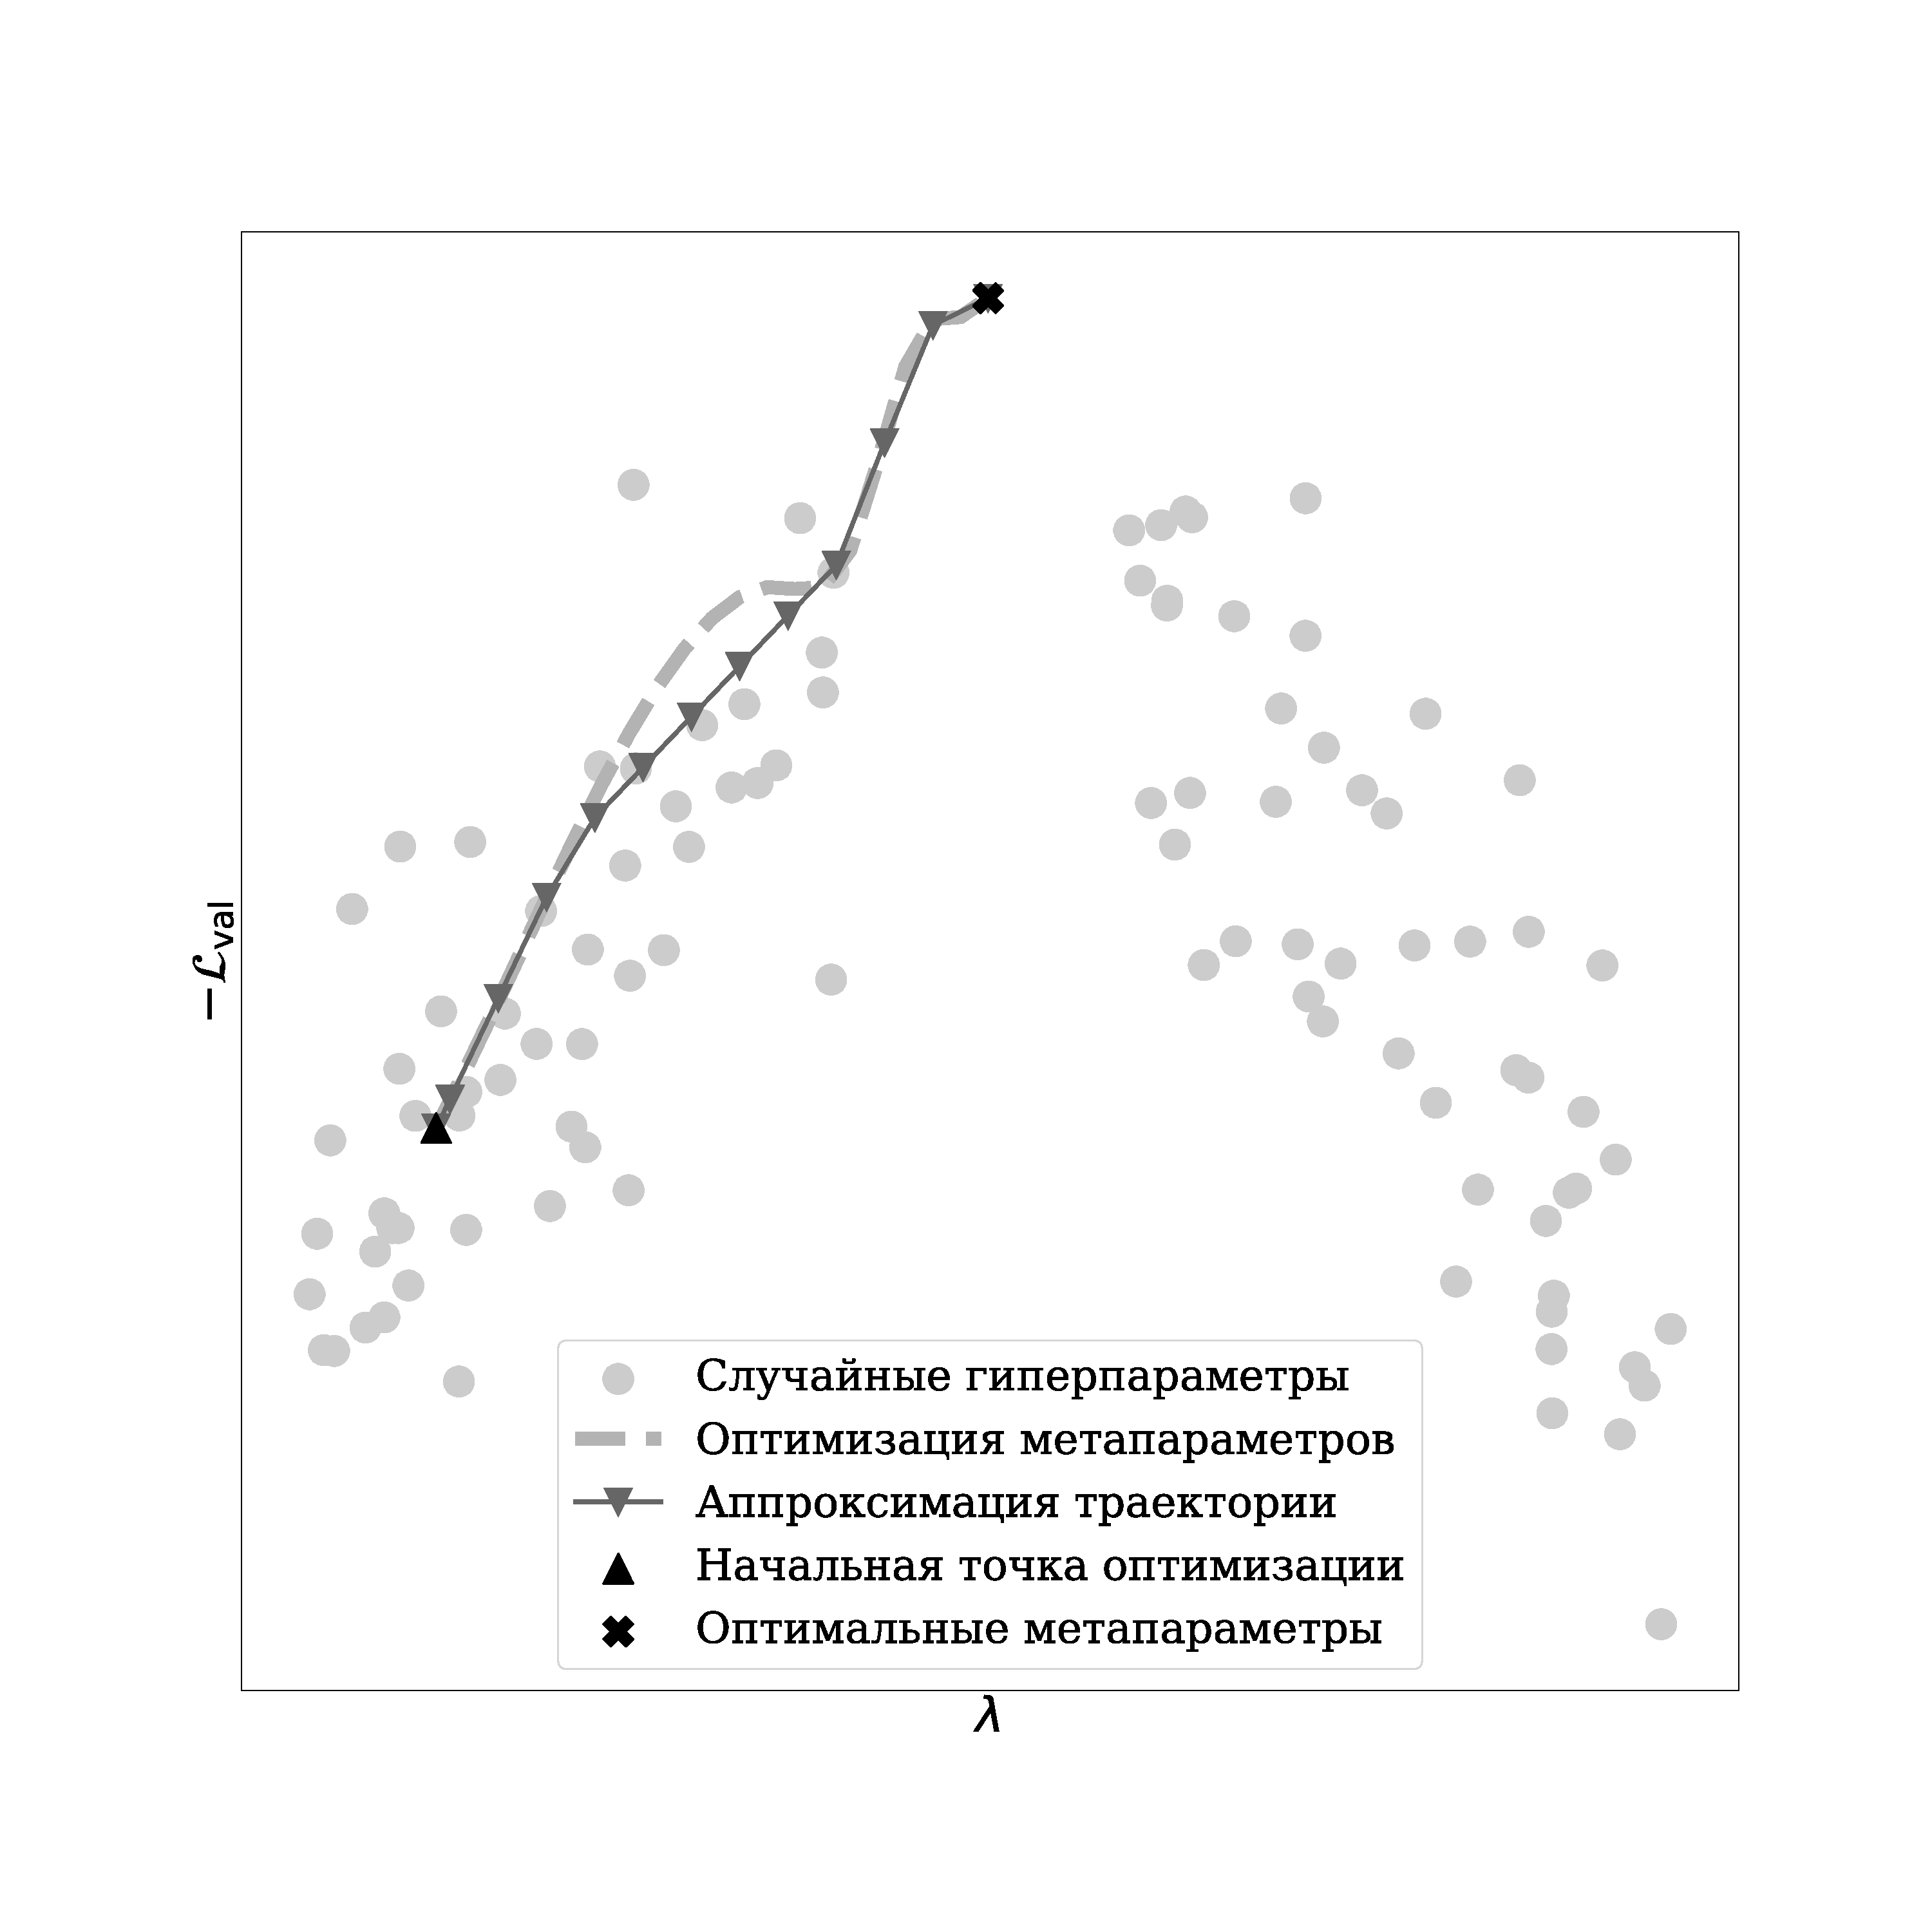
\includegraphics[width=0.7\linewidth]{ait-utf/trajectory_rus.pdf}}
    \caption{Схема работы предложенного метода: вместо непосредственной оптимизации значений метапараметра $\lambda$ предлагается аппроксимировать траекторию оптимизации с помощью линейных моделей для достижения минимума функции потерь на валидационной части выборки $\mathcal{L}_\text{val}$. Случайные метапараметры не являются точками минимума функции $\mathcal{L}_\text{val}$ и доставляют субоптимальное качество модели.}
    \label{fig:trajectory}
\end{figure}

Предлагается рассматривать задачу оптимизации метапараметров как двухуровневую задачу оптимизации. На первом уровне оптимизируются параметры модели, на втором --- метапараметры~\cite{journals/corr/LuketinaBR15,journals/anor/BakhteevS20,journals/corr/MaclaurinDA15}. Жадный градиентный метод для решения двухуровневой задачи описан в~\cite{journals/corr/LuketinaBR15}. В~\cite{journals/anor/BakhteevS20} проанализированы различные градиентные методы и случайный поиск. 
В данной работе анализируется подход к оптимизации и предсказанию метапараметров, полученных после применения градиентных методов. Из Таблицы~\ref{table:compl} можно увидеть, что для больших задач предпочтительны градиентные методы оптимизации метапараметров. Тем не менее, даже с применением жадного алгоритма оптимизации метапараметров с разностной аппрокисимацией, оптимизация метапараметров становится значительно требовательнее к вычислительным ресурсам, что было продемонстрировано в работе~\cite{liu2018darts}. Для уменьшения затрат на оптимизацию в настоящей работе проводится анализ траектории оптимизации метапараметров и предсказывается ее значение с помощью линейных моделей. Этот метод проиллюстрирован на Рис. \ref{fig:trajectory}. Данный метод оценивается и сравнивается с другими методами оптимизации метапараметров на выборках изображений CIFAR-10~\cite{krizhevsky2009learning}, Fashion-MNIST \cite{journals/corr/abs-1708-07747} и синтетической выборке. 

%%%%%%%%%%%%%%%%%%%%%%%%%%%%%%%%%%%%%%%%%%%%%
% Вклад данной работы:
% \begin{enumlist}
%     \item сравниваются два подхода к оптимизации метапараметров в задаче дистилляции: стохастический и градиентный;
    
%     \item предлагается улучшение градиентной оптимизации с целью уменьшения вычислительной сложности оптимизации;
    
%     \item приведен теоретический анализ предложенного метода и оценено его качество для задачи дистилляции.
% \end{enumlist}
%%%%%%%%%%%%%%%%%%%%%%%%%%%%%%%%%%%%%%%%%%%%%

\section{Постановка задачи}

Решается задача классификации вида:

$$
    \mathfrak{D} = \{(\mathbf{x}_i, \mathbf{y}_i)\}_{i=1}^{m},\; \mathbf{x}_i \in \mathbb{R}^n,\; \mathbf{y}_i \in \mathbb{Y} = \{\mathbf{e}_k | k = \overline{1, K}\},
$$
% \{[0, \dots, 0, \underset{k}{1}, 0, \dots, 0]^\top | k = \overline{1, K}\},

\noindent
где $\mathbf{e}_k$ --- $k$-й столбец единичной матрицы, $\mathbf{y}_i$ --- вектор с единицей на месте класса $\mathbf{x}_i$.

Разделим выборку на два подмножества $\mathfrak{D}$: $\mathfrak{D} = \mathfrak{D}_\text{train} \sqcup \mathfrak{D}_\text{val}.$ Подмножество $\mathfrak{D}_\text{train}$ будем использовать для оптимизации параметров модели, а подмножество $\mathfrak{D}_\text{val}$ --- для оптимизации метапараметров.

Рассмотрим модель-учителя $\mathbf{f}(\mathbf{x})$, которая была обучена на выборке $\mathfrak{D}_\text{train}$. Оптимизируем модель-ученика $\mathbf{g}(\mathbf{x}, \mathbf{w})$, $\mathbf{w} \in \mathbb{R}^s$ путем переноса знаний модели-учителя. Определим данную задачу формально.

\begin{definition}
Пусть функция~$D: \mathbb{R}^s \to \mathbb{R}_{+}$ задает расстояние между моделью-учеником~$\mathbf{g}$ и моделью-учителем~$\mathbf{f}$. Назовем $D$-дистилляцией модели-ученика такую задачу оптимизации параметров модели-ученика, которая минимизирует функцию~$D$.
\end{definition}

Определим функцию потерь $\mathcal{L}_\text{train}$, которая учитывает перенос знаний от модели $\mathbf{f}$ к модели $\mathbf{g}$:


\begin{multline*}
    \mathcal{L}_\text{train}(\mathbf{w}, \boldsymbol{\lambda}) = -\lambda_1\sum\limits_{(\mathbf{x}, \mathbf{y}) \in \mathfrak{D}_\text{train}}\underbrace{\sum\limits_{k=1}^{K}y_k\log \frac{e^{\mathbf{g}(\mathbf{x}, \mathbf{w})_k}}{\sum\limits_{j=1}^{K}e^{\mathbf{g}(\mathbf{x}, \mathbf{w})_j}}}_{\text{слагаемое классификации}} \\- (1 - \lambda_1)\sum\limits_{(\mathbf{x}, y) \in \mathfrak{D}_\text{train}}\underbrace{\sum\limits_{k=1}^{K}\frac{e^{\mathbf{f}(\mathbf{x})_k/T}}{\sum\limits_{j=1}^{K}e^{\mathbf{f}(\mathbf{x})_j/T}}\log \frac{e^{\mathbf{g}(\mathbf{x}, \mathbf{w})_k/T}}{\sum\limits_{j=1}^{K}e^{\mathbf{g}(\mathbf{x}, \mathbf{w})_j/T}}}_{\text{слагаемое дистилляции}},
\end{multline*}

\noindent
где~$y_k$ --- это $k$-я компонента вектора ответов,~$T$ --- параметр температуры в задаче дистилляции. Температура $T$ имеет следующие свойства:

\begin{enumerate}
    \item если $T \rightarrow 0$, то получаем единичный вектор $\Bigl\{\frac{e^{\mathbf{g}(\mathbf{x}, \mathbf{w})_k/T}}{\sum\limits_{j=1}^{K}e^{\mathbf{g}(\mathbf{x}, \mathbf{w})_j/T}}\Bigr\}_{k=1}^K$;
    \item если $T \rightarrow \infty$, то получаем вектор с равными вероятностями.
\end{enumerate}

%Покажем, что дивергенция Кульбака-Лейблера является частным случаем $D$-дистилляции.
Покажем, что оптимизация $\mathcal{L}_\text{train}$ является $D$-дистилляцией при $\lambda_1 = 0$.

\begin{proposition}
Если~$\lambda_1 = 0$, то оптимизация функции потерь \eqref{train_loss}, является $D$-дистилляцией с $D = D_{KL}\left(\sigma\left(\mathbf{f}(\mathbf{x})/T\right), \sigma\left(\mathbf{g}(\mathbf{x}, \mathbf{w})/T\right)\right)$, где $\sigma$ --- это функция $\text{softmax} = \frac{e^{x_i}}{\sum\limits_{j=1}^Ke^{x_j}}$.
\end{proposition}

\begin{proof}
При~$\lambda_1 = 0$ имеем:

\begin{multline}
    \mathcal{L}_\text{train}(\mathbf{w}, \boldsymbol{\lambda}) = \sum\limits_{(\mathbf{x}, y) \in \mathfrak{D}_\text{train}}\sum\limits_{k=1}^{K}\frac{e^{\mathbf{f}(\mathbf{x})_k/T}}{\sum\limits_{j=1}^{K}e^{\mathbf{f}(\mathbf{x})_j/T}}\log \frac{e^{\mathbf{g}(\mathbf{x}, \mathbf{w})_k/T}}{\sum\limits_{j=1}^{K}e^{\mathbf{g}(\mathbf{x}, \mathbf{w})_j/T}} \\= D_{KL}\left(\sigma(\mathbf{f}(\mathbf{x})/T), \sigma(\mathbf{g}(\mathbf{x}, \mathbf{w})/T)\right).
    \label{train_loss}
\end{multline}

Функция $D_{KL}\left(\sigma\left(\mathbf{f}/T\right), \sigma\left(\mathbf{g}/T\right)\right)$ определяет расстояние между логитами модели $\mathbf{f}$ и модели $\mathbf{g}$. Получаем, что определение $D$-дистилляции выполняется. 

\end{proof}

% $\hspace{12.3 cm}\Box$

Определим множество метапараметров~$\boldsymbol{\lambda}$ как вектор, компонентами которого являются коэффициент $\lambda_1$ перед слагаемыми в $\mathcal{L}_\text{train}$ и температура~$T$:

\[\boldsymbol{\lambda} = [\lambda_1, T].\]
Определим двухуровневую задачу:
\begin{equation} \label{eq:opt_hyp}
    \hat{\boldsymbol{\lambda}} = \arg\min\limits_{\boldsymbol{\lambda} \in \mathbb{R}^2} \mathcal{L}_\text{val}(\hat{\mathbf{w}}, \boldsymbol{\lambda}),
\end{equation}
\begin{equation} \label{eq:opt_param}
    \hat{\mathbf{w}} = \arg\min\limits_{\mathbf{w} \in \mathbb{R}^s} \mathcal{L}_\text{train}(\mathbf{w}, \boldsymbol{\lambda}),
\end{equation}
где $\mathcal{L}_\text{val}$ --- это функция потерь на валидации:

$$
     \mathcal{L}_\text{val}(\mathbf{w}, \boldsymbol{\lambda}) = - \sum\limits_{(\mathbf{x}, y) \in \mathfrak{D}_\text{val}}\sum\limits_{k=1}^{K}y^k\log \frac{e^{\mathbf{g}(\mathbf{x}, \mathbf{w})_k/T_\text{val}}}{\sum\limits_{j=1}^Ke^{\mathbf{g}(\mathbf{x}, \mathbf{w})_j/T_\text{val}}},
$$
метапараметр $T_\text{val}$ определяет температуру в валидационной функции потерь. Его значение выбрано вручную и не является предметом оптимизации. 


\section{Градиентная оптимизация метапараметров}

Одним из методов оптимизации метапараметров является использование градиентных методов. Ниже приведена схема их применения и подход к оптимизации траектории метапараметров.

\begin{definition} 
Определим \textit{оператор оптимизации} как алгоритм $U$, который выбирает вектор параметров модели $\mathbf{w}^\prime$ используя значения параметров на предыдущем шаге $\mathbf{w}$.
\end{definition}

Оптимизируем параметры $\mathbf{w}$ используя $\eta$ шагов оптимизации:

$$
    \hat{\mathbf{w}} = U \circ U \circ \dots \circ U(\mathbf{w}_0, \boldsymbol{\lambda}) = U^\eta(\mathbf{w}_0, \boldsymbol{\lambda}),
$$

\noindent
где $\mathbf{w}_0$ --- начальное значение вектора параметров $\mathbf{w}$, $\boldsymbol{\lambda}$ --- множество метапараметров.

Переформулируем оптимизационную задачу, используя определение оператора $U$:

$$
    \hat{\boldsymbol{\lambda}} = \arg\min\limits_{\boldsymbol{\lambda} \in \mathbb{R}^2} \mathcal{L}_\text{val}\bigl(U^\eta(\mathbf{w}_0, \boldsymbol{\lambda})\bigr).
$$

Решим оптимизационную задачу \eqref{eq:opt_hyp} и \eqref{eq:opt_param} с помощью оператора градиентного спуска:
$$
    U(\mathbf{w}, \boldsymbol{\lambda}) = \mathbf{w} - \gamma\nabla\mathcal{L}_\text{train}(\mathbf{w}, \boldsymbol{\lambda}),
$$
где $\gamma$ --- длина шага градиентного спуска. Для оптимизации метапараметров используется жадный градиентный метод, который зависит только от значения параметров $\mathbf{w}$ на предыдущем шаге. На каждой итерации получим следующее значение метапараметров:

\begin{equation}
    \boldsymbol{\lambda}^\prime = \boldsymbol{\lambda} - \gamma_{\boldsymbol{\lambda}}\nabla_{\boldsymbol{\lambda}}\mathcal{L}_\text{val}(U(\mathbf{w}, \boldsymbol{\lambda}), \boldsymbol{\lambda}) = \boldsymbol{\lambda}\\ - \gamma_{\boldsymbol{\lambda}}\nabla_{\boldsymbol{\lambda}}\mathcal{L}_\text{val}(\mathbf{w} - \gamma\nabla\mathcal{L}_\text{train}(\mathbf{w}, \boldsymbol{\lambda}), \boldsymbol{\lambda}).
    \label{eq:hyp_alg}
\end{equation}

В данной работе используется численная разностная аппроксимация для данной процедуры оптимизации~\cite{liu2018darts}:

$$
\frac{d\mathcal{L}_\text{val}(\mathbf{w}^\prime, \boldsymbol{\lambda})}{d\boldsymbol{\lambda}} = \nabla_{\boldsymbol{\lambda}}\mathcal{L}_\text{val}(\mathbf{w}^\prime, \boldsymbol{\lambda})  - \gamma\nabla^2_{\boldsymbol{\lambda}, \mathbf{w}^\prime}\mathcal{L}_\text{val}(\mathbf{w}^\prime, \boldsymbol{\lambda})\nabla_{\mathbf{w}^\prime}\mathcal{L}_\text{val}(\mathbf{w}^\prime, \boldsymbol{\lambda}),
$$

$$
\nabla^2_{\boldsymbol{\lambda}, \mathbf{w}^\prime}\mathcal{L}_\text{val}(\mathbf{w}^\prime, \boldsymbol{\lambda})\nabla_{\mathbf{w}^\prime}\mathcal{L}_\text{val}(\mathbf{w}^\prime, \boldsymbol{\lambda}) \approx \frac{\nabla_{\boldsymbol{\lambda}}\mathcal{L}_\text{val}(\mathbf{w}^+, \boldsymbol{\lambda}) - \nabla_{\boldsymbol{\lambda}}\mathcal{L}_\text{val}(\mathbf{w}^-, \boldsymbol{\lambda})}{2\varepsilon},
$$

$$
\boldsymbol{\lambda}^\prime \approx \boldsymbol{\lambda} - \gamma_{\boldsymbol{\lambda}}\nabla_{\boldsymbol{\lambda}}\mathcal{L}_\text{val}(\mathbf{w}^\prime, \boldsymbol{\lambda})  + \gamma\frac{\nabla_{\boldsymbol{\lambda}}\mathcal{L}_\text{val}(\mathbf{w}^+, \boldsymbol{\lambda}) - \nabla_{\boldsymbol{\lambda}}\mathcal{L}_\text{val}(\mathbf{w}^-, \boldsymbol{\lambda})}{2\varepsilon}
$$

\noindent
где $\mathbf{w}^\prime = \mathbf{w} - \gamma\nabla\mathcal{L}_\text{train}(\mathbf{w}, \boldsymbol{\lambda})$, $\mathbf{w}^\pm = \mathbf{w}^\prime \pm \varepsilon \nabla_{\mathbf{w}^\prime}\mathcal{L}_\text{val}(\mathbf{w}^\prime, \boldsymbol{\lambda})$, $\varepsilon$ --- некоторая заданная константа.

Для дальнейшего уменьшения стоимости оптимизации предлагается аппроксимировать траекторию оптимизации метапараметров. Траектория предсказывается с помощью линейных моделей, которые используются периодически после заданного числа итераций $e_1$. После этого линейная модель используется для предсказания метапараметров на протяжении $e_2$ итераций:

\begin{equation}
     \boldsymbol{\lambda}^\prime = 
     \boldsymbol{\lambda} + \mathbf{c}^{\top}\begin{pmatrix}z\\1\end{pmatrix},
     \label{eq:linear}
\end{equation}
где $\mathbf{c}$ --- это вектор параметров линейной модели, оптимизированный с помощью метода наименьших квадратов, $z$ --- число итераций оптимизации. Алгоритм предложенного метода приведен на Рис.~\ref{algo}.


% \begin{figure}

% \center{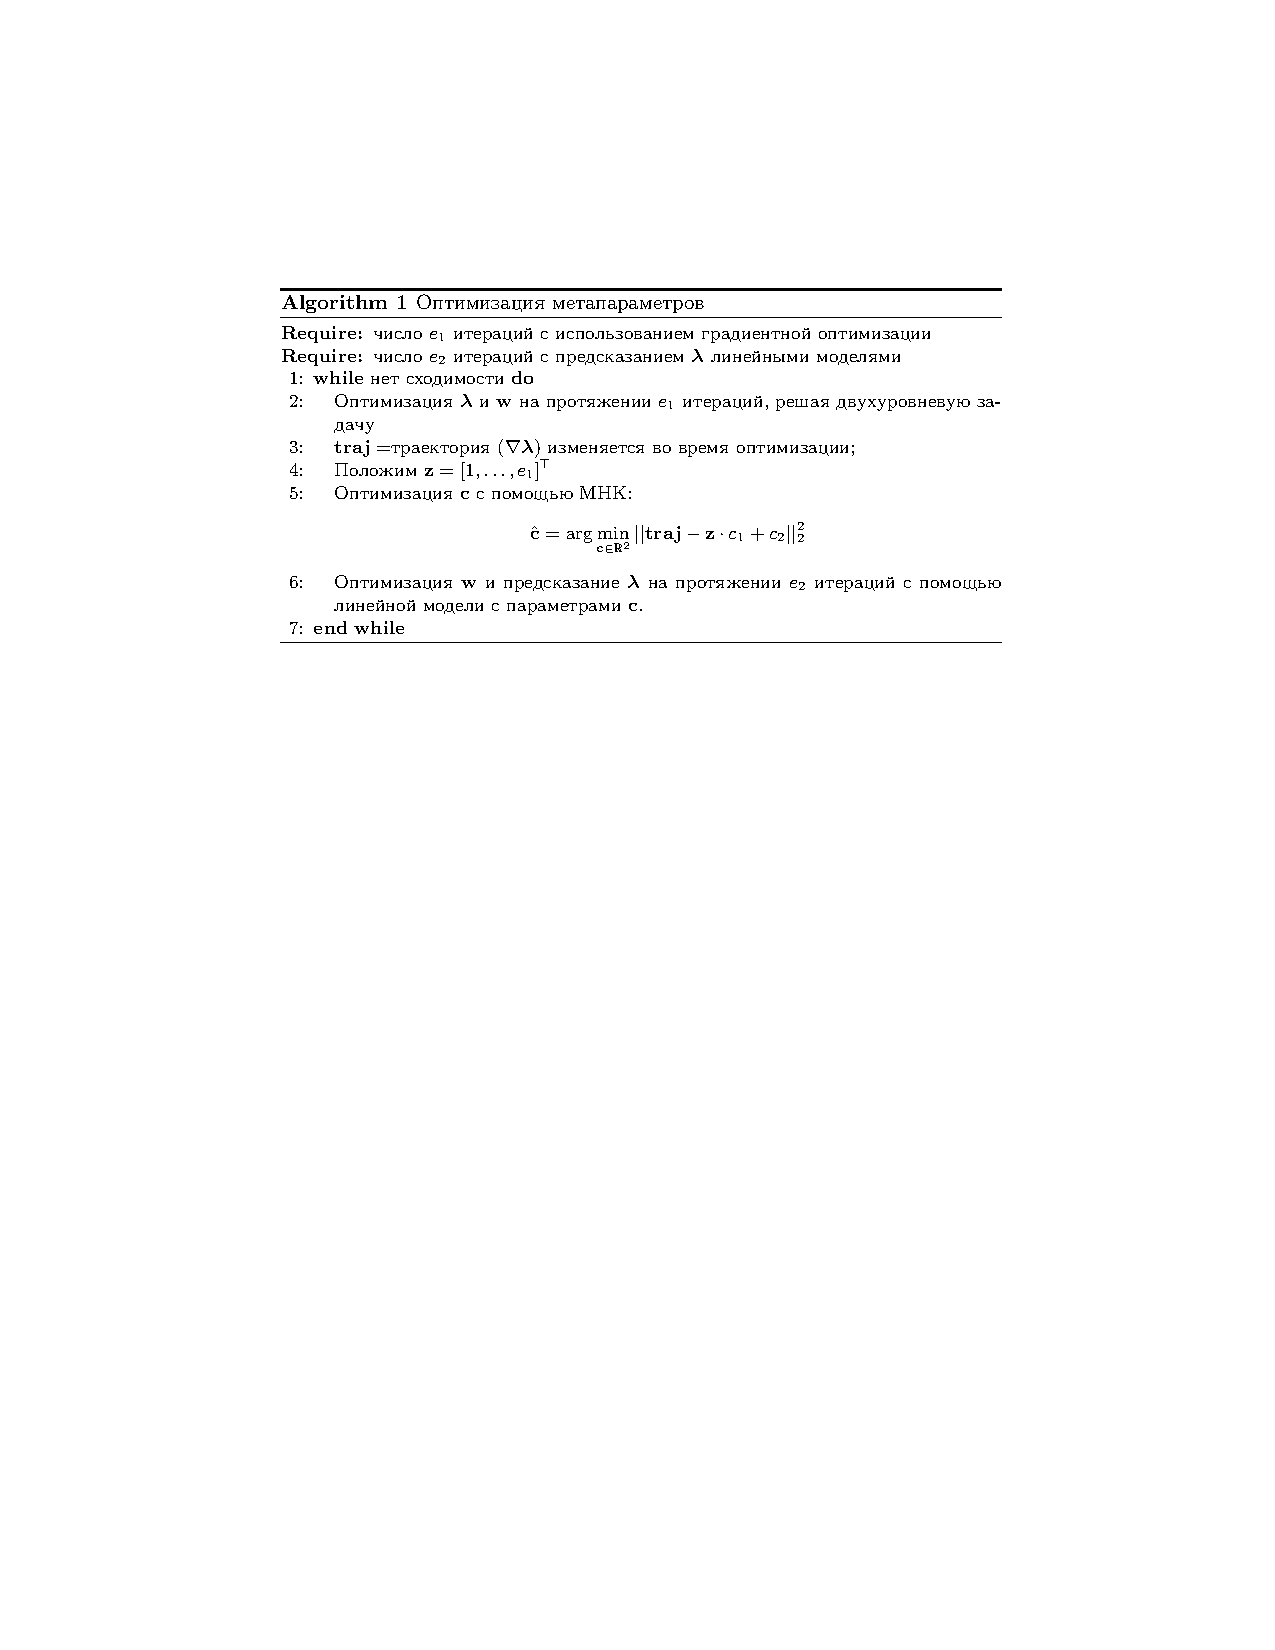
\includegraphics[width=\linewidth]{ait-utf/alg.pdf}}

% \caption{Алгоритм для предложенного метода.} \label{algo}

% \end{figure}

%----------------------------------------------
% \begin{algorithm}[(Оптимизация метапараметров)] \label{algo}\

% \textbf{Дано:}
% \begin{itemize}
%     \item число $e_1$ итераций с использованием градиентной оптимизации;
%     \item  число $e_2$ итераций с предсказанием $\boldsymbol{\lambda}$ линейными моделями.
% \end{itemize}

% Пока не достигнута сходимость:
% \begin{enumlist}[.]
%     \item Оптимизация $\boldsymbol{\lambda}$ и $\mathbf{w}$ на протяжении $e_1$ итераций, решая двухуровневую задачу
%     \item $\textbf{traj} = $траектория $(\nabla \boldsymbol{\lambda})$ изменяется во время оптимизации;
%     \item Положим $\mathbf{z} = [1,\dots,e_1]^\mathsf{T}$
%     \item Оптимизация $\mathbf{c}$ с помощью МНК: 
%   $$\hat{\mathbf{c}} = \arg\min_{\mathbf{c} \in \mathbb{R}^2} ||\textbf{traj} - \mathbf{z}\cdot c_1 + c_2||_2^2$$
%   \item Оптимизация $\mathbf{w}$ и предсказание $\boldsymbol{\lambda}$ на протяжении $e_2$ итераций с помощью линейной модели с параметрами $\mathbf{c}$.
% \end{enumlist}

% \end{algorithm}
% ----------------------------------------------
\begin{figure}

\begin{algorithm}[H]
\caption{Оптимизация метапараметров}
\begin{algorithmic}[1]

 %\renewcommand{\algorithmicrequire}{\mathbf{Input:}}
 %\renewcommand{\algorithmicensure}{\mathbf{Output:}}
 \REQUIRE число $e_1$ итераций с использованием градиентной оптимизации
 \REQUIRE число $e_2$ итераций с предсказанием $\boldsymbol{\lambda}$ линейными моделями
 %\REQUIRE in
 %\ENSURE  out
  \WHILE {нет сходимости}
  \STATE Оптимизация $\boldsymbol{\lambda}$ и $\mathbf{w}$ на протяжении $e_1$ итераций, решая двухуровневую задачу
  \STATE $\textbf{traj} = $траектория $(\nabla \boldsymbol{\lambda})$ изменяется во время оптимизации;
  \STATE Положим $\mathbf{z} = [1,\dots,e_1]^\mathsf{T}$
  \STATE Оптимизация $\mathbf{c}$ с помощью МНК: 
  $$\hat{\mathbf{c}} = \arg\min_{\mathbf{c} \in \mathbb{R}^2} ||\textbf{traj} - \mathbf{z}\cdot c_1 + c_2||_2^2$$
  \STATE Оптимизация $\mathbf{w}$ и предсказание $\boldsymbol{\lambda}$ на протяжении $e_2$ итераций с помощью линейной модели с параметрами $\mathbf{c}$.
  \ENDWHILE

 \end{algorithmic}
 \end{algorithm}
 
 \caption{Алгоритм для предложенного метода.}
 \label{algo}

 \end{figure}

Диаграмма на Рис.~\ref{fig:scheme} описывает полученный метод оптимизации. Параметры модели оптимизируются на первом уровне двухуровневой оптимизационной задачи с помощью подмножества $\mathfrak{D}_\text{train}$ и функции потерь $\mathcal{L}_{\text{train}}$. Метапараметры оптимизируются на втором уровне с помощью подмножества $\mathfrak{D}_\text{val}$ и функции потерь $\mathcal{L}_\text{val}$. На протяжении $e_1$ итераций метапараметры оптимизируются с помощью метода стохастического градиентного спуска. На протяжении $e_2$ итераций предсказываются с помощью линейных моделей.

\begin{figure}
$$
\xymatrix{
\mathbf{w} - \gamma\nabla\mathcal{L}_\text{train}(\mathbf{w}, \boldsymbol{\lambda})\ar[r] & \hat{\mathbf{w}}, \mathbf{x}\ar[r]^{\mathbf{g}} & \hat{y}\ar[r] & \mathcal{L}_\text{train}(\mathbf{w}, \boldsymbol{\lambda})\ar@/_2pc/[lll]\\
t\ar[r] & i\ar[r] & (\mathbf{x}, \mathbf{y})\ar[r]\ar[dr] & \mathfrak{D}_\text{train}\ar[u]\\
 &  &  & \mathfrak{D}_\text{val}\ar[d]_{e_1}\\
 &  &  & \mathcal{L}_{\text{val}}(\boldsymbol{\lambda})\ar[dll]\\
 & \boldsymbol{\lambda} - \gamma_{\boldsymbol{\lambda}}\nabla_{\boldsymbol{\lambda}}\mathcal{L}_\text{val}(U(\mathbf{w}, \boldsymbol{\lambda}), \boldsymbol{\lambda})\ar[rr] &  & \boldsymbol{\lambda}^\prime\ar[u]\ar@/_0.5pc/[d]_{e_2}\ar@/_2pc/[uuuu]\\
 &  &  & \boldsymbol{\lambda}^\prime + \mathbf{c}^\top\textbf{z}\ar@/_0.5pc/[u]
}
$$
\caption{Схема оптимизации метапараметров.}
\label{fig:scheme}

\end{figure}

%-----------------
% \begin{figure}

% \center{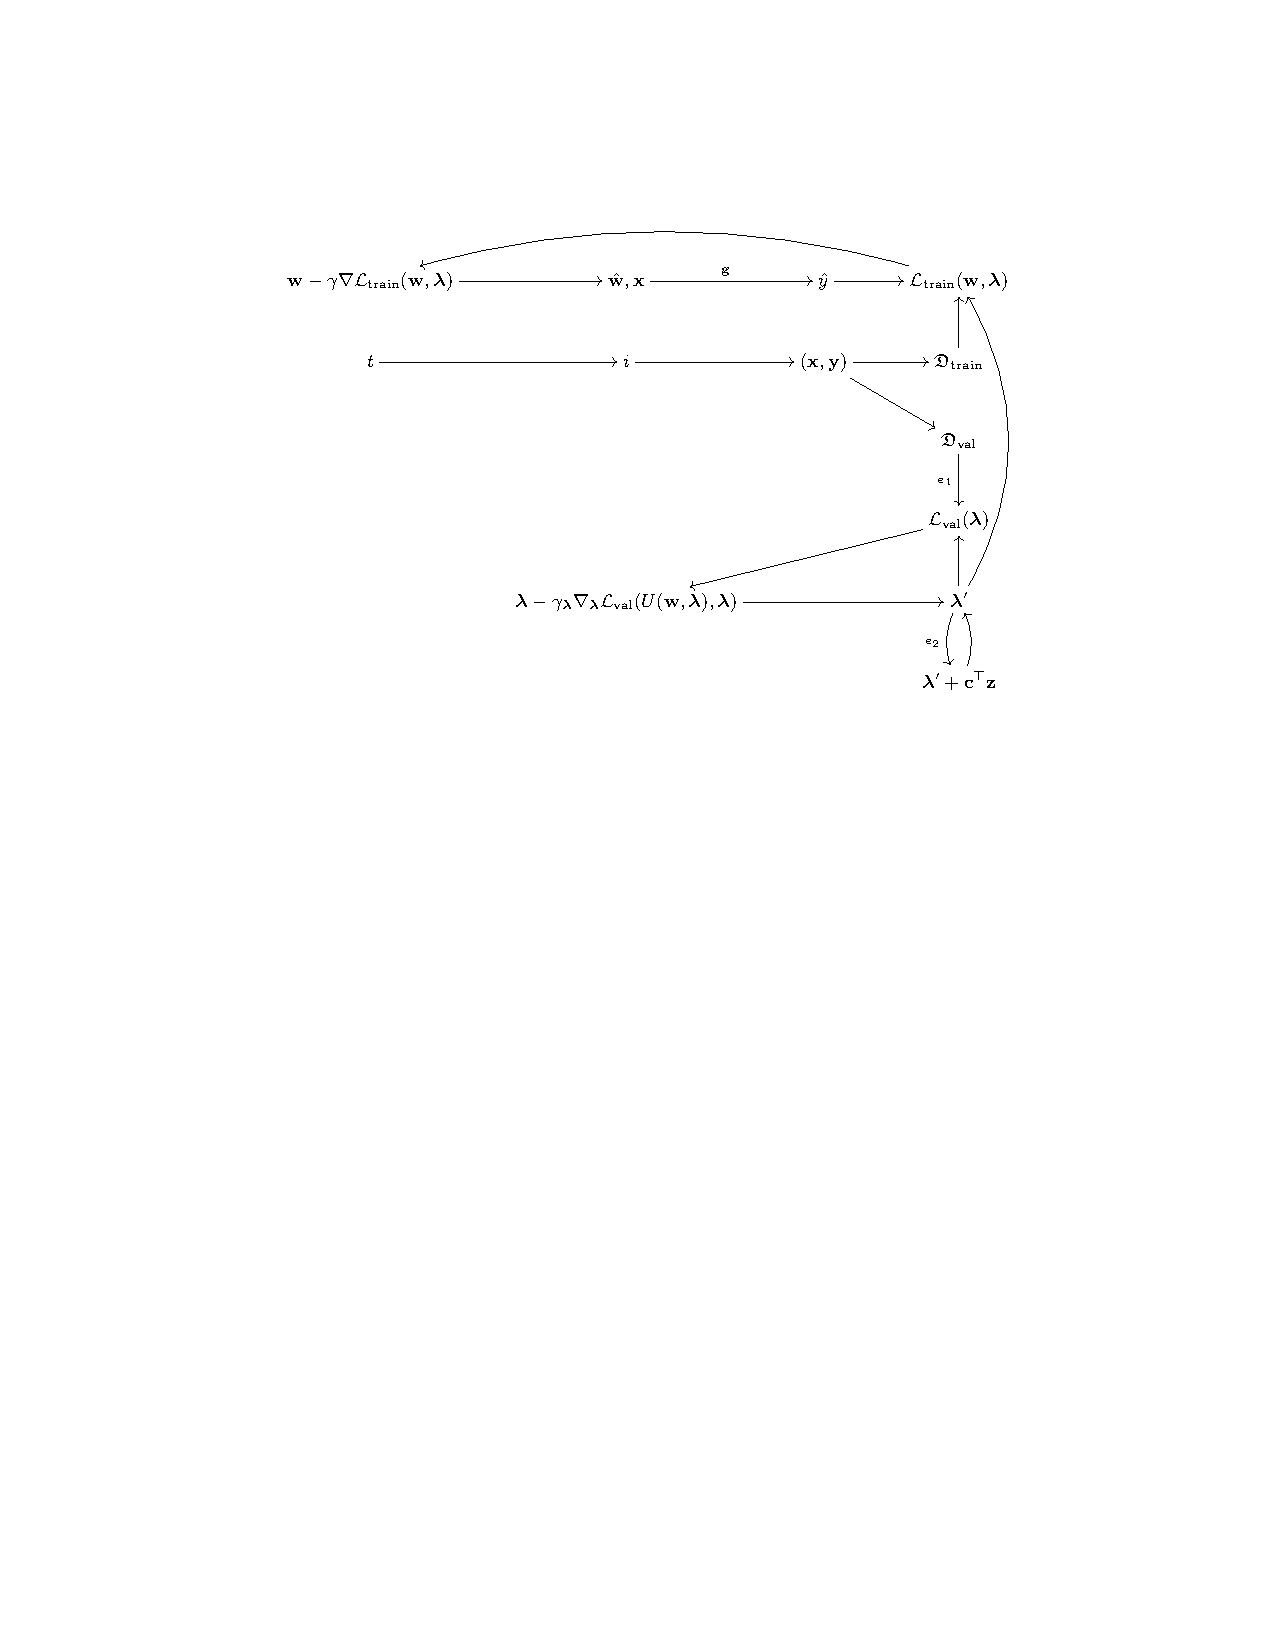
\includegraphics[width=\linewidth]{ait-utf/scheme.pdf}}
% \caption{Схема оптимизации метапараметров.}
% \label{fig:scheme}

% \end{figure}
%------------------

% \begin{itemize}
% \item[] $f$ is the forecasting model,
% \item[] $S$ is the criterion,
% \item[] $T$ is an optimization algorithm,
% \item[] $\hat{\textbf{w}}$ is some solution,
% \end{itemize}

% \begin{equation*}
% \hat{\textbf{w}}= \arg\min S(\textbf{w}|y,f).
% \end{equation*}

\noindent
%Следующая теорема доказывает корректность аппроксимации линейными моделями.
Следующая теорема доказывает корректность предложенной аппроксимации для простого случая: когда параметры $\mathbf{w}$ модели $\mathbf{g}$ достигли оптимума задачи~\eqref{eq:opt_param}, гессиан $\mathbf{H} = \nabla_{\mathbf{w}}^2 \mathcal{L}_\textnormal{train}$ является единичной матрицей, и оптимизация метапараметров ведется в области, в которой градиент метапараметров можно аппроксимировать константой. Отметим, что в общем случае, данные условия при оптимизации моделей глубокого обучения не выполняются. В работах~\cite{journals/corr/LuketinaBR15,Vatanen} было показано, что использование методов нормализации промежуточных представлений выборки под действием нелинейных функций, входящих в модель глубокого обучения, приближает гессиан функции потерь к единичному. Анализ качества градиентной оптимизации метапараметров для случая, когда параметры модели не достигли оптимума, приведен в~\cite{journals/corr/Pedregosa16}.

\begin{theorem}
Если функция $\mathcal{L}_{\text{train}}(\mathbf{w}, \boldsymbol{\lambda})$ является гладкой и выпуклой, и ее гессиан $\mathbf{H} = \nabla_{\mathbf{w}}^2 \mathcal{L}_\textnormal{train}$ является единичной матрицей, $\mathbf{H} = \mathbf{I},$ а также если параметры $\mathbf{w}$ равны $\mathbf{w}^*$, где $\mathbf{w}^*$ --- точка локального минимума для текущего значения $\boldsymbol{\lambda},$ тогда жадный алгоритм~\eqref{eq:hyp_alg} находит оптимальное решение двухуровневой задачи. Если существует область $\mathcal{D} \in \mathbb{R}^2$ в пространстве метапараметров, такая что градиент метапараметров может быть аппроксимирован константой, то оптимизация является линейной по метапараметрам.
\end{theorem}

\begin{proof} 
В работе \cite{journals/corr/Pedregosa16} была выведена формула для $\nabla_{\boldsymbol{\lambda}}\mathcal{L}_\text{val} = \nabla_{\boldsymbol{\lambda}}\mathcal{L}_\text{val}(U(\mathbf{w}, \boldsymbol{\lambda}))$ в случае, если $\mathcal{L}_\text{train}(\textbf{w}, \boldsymbol{\lambda})$ является гладкой и выпуклой, и найдена $\mathbf{w}^*$ --- точка локального минимума для текущего значения $\boldsymbol{\lambda}$:

$$
    \nabla_{\boldsymbol{\lambda}}\mathcal{L}_\text{val}(\boldsymbol{\lambda}) = \nabla_{\boldsymbol{\lambda}}\mathcal{L}_\text{val} - (\nabla_{\textbf{w}, \boldsymbol{\lambda}}^2\mathcal{L}_\text{train})^\top(\nabla_{\textbf{w}}^2\mathcal{L}_\text{train})^{-1}\nabla_{\textbf{w}}\mathcal{L}_\text{val}.
$$

Эта формула упрощается исключением первого слагаемого, так как функция $\mathcal{L}_\text{val}$ явно не зависит от метапараметров:

$$
    \nabla_{\boldsymbol{\lambda}}\mathcal{L}_\text{val}(\boldsymbol{\lambda}) = - (\nabla_{\textbf{w}, \boldsymbol{\lambda}}^2\mathcal{L}_\text{train})^\top(\nabla_{\textbf{w}}^2\mathcal{L}_\text{train})^{-1}\nabla_{\textbf{w}}\mathcal{L}_\text{val}.
$$

Если $\nabla_{\textbf{w}}^2 \mathcal{L}_\text{train}$ равен единичной матрице, то жадный алгоритм дает оптимум двухуровневой задачи в том случае, если его шаг выражается следующей формулой~\cite{journals/corr/LuketinaBR15}:

$$
    \boldsymbol{\lambda}_{t+1} = \boldsymbol{\lambda}_{t} + \eta_1(\nabla_{\textbf{w}, \boldsymbol{\lambda}}^2\mathcal{L}_\text{train})^\top\nabla_{\textbf{w}}\mathcal{L}_\text{val}.
$$

Также заменим $\nabla_{\textbf{w}}^2 \mathcal{L}_\text{train}$ на единичную матрицу.

Вернемся к упрощенной формуле градиента:

$$\nabla_{\boldsymbol{\lambda}}\mathcal{L}_\text{val}(\boldsymbol{\lambda}) = - (\nabla_{\textbf{w}, \boldsymbol{\lambda}}^2\mathcal{L}_\text{train})^\top\nabla_{\textbf{w}}\mathcal{L}_\text{val}.$$

Предположим, что существует область $\mathcal{D}$, в которой $\nabla_{\boldsymbol{\lambda}}\mathcal{L}_\text{val}(\boldsymbol{\lambda})$ равен константному вектору

\[\nabla_{\boldsymbol{\lambda}}\mathcal{L}_\text{val}(\boldsymbol{\lambda}) \approx \begin{pmatrix} a_1\\ a_2\end{pmatrix}.\]

Тогда в $\mathcal{D}$ шаг оптимизации можно представить в виде
$$
    \boldsymbol{\lambda}_{t+1} = \boldsymbol{\lambda}_{t} - \gamma_{\boldsymbol{\lambda}}\begin{pmatrix} a_1\\ a_2\end{pmatrix},
$$
\noindent
и имеет вид, аналогичный~\eqref{eq:linear}.
\end{proof}



\section{Вычислительный эксперимент}

Целью эксперимента является оценка качества предложенного метода дистилляции и анализ полученных моделей и их метапараметров. Метод оценивался на синтетической выборке, а также выборках CIFAR-10 и Fashion-MNIST.%~\footnote{Исходный код вычислительного эксперимента доступен по ссылке: https://github.com/Intelligent-Systems-Phystech/2021-Project-84} 
На выборке CIFAR-10 было проведено два вида экспериментов: на всей выборке, $|\mathfrak{D}_\text{train}|=50000$, и на уменьшенной обучающей выборке, $|\mathfrak{D}_\text{train}|=12800$. 

Были проанализированы следующие методы оптимизации метапараметров:
\begin{enumlist}
    \item оптимизация без дистилляции;
    \item оптимизация со случайной инициализацией метапараметров. Метапараметры порождаются из равномерного распределения $$\lambda_1 \sim \mathcal{U}(0;1), \quad T \sim \mathcal{U}(0.1, 10).$$
    \item оптимизация с ``наивным'' назначением метапараметров:  $$\lambda_1 = 0.5, T = 1;$$
    \item градиентная оптимизация;
    \item предложенный метод с $e_1=e_2=10.$
    \item оптимизация с помощью вероятностной модели. Для данного типа оптимизации использовалась библиотека hyperopt~\cite{bergstra2013making}, в которой реализована оптимизация с помощью метода парзеновского окна. Для этого метода проводилось 5 запусков перед итоговым предсказанием метапараметров.
\end{enumlist}

Для методов 1-3 использовалась вся обучающая выборка $\mathfrak{D}$. Для методов 4-6 выборка разбивалась на обучение, валидацию, контроль $\mathfrak{D} = \mathfrak{D}_\text{train} \sqcup \mathfrak{D}_\text{val} \sqcup \mathfrak{D}_\text{test}.$

В качестве внешнего критерия качества была использована метрика accuracy:
$$
    \text{accuracy} = \frac{1}{m}\sum\limits_{i=1}^m [\mathbf{g}(\mathbf{x}_i, \mathbf{w}) = y_i],
$$

Для всех экспериментов порождение начальных значений метапараметров происходило следующим образом: 
$$\lambda_1 \sim \mathcal{U}(0,1),\quad \log_{10} T \sim \mathcal{U}(-1, 1).$$ 

Для каждого эксперимента проводилось 10 запусков, затем результаты усреднялись. Код эксперимента доступен в~\cite{source_code}.

Итоговые результаты представлены в Таблице~\ref{table:results}. Зависимость точности от номера итерации на синтетической выборке и уменьшенной версии CIFAR-10 изображена на Рис.~\ref{fig:accuracy}.

\begin{table}[]

\caption{Результаты эксперимента. Числа в скобках являются максимальным полученным значением точности в конкретном эксперименте.}

\label{table:results}
\footnotesize
\centering
\begin{tabularx}{\textwidth}{|X|X|X|X|X|X}
\cline{1-5}
Метод                      & Синтетическая выборка & Fashion-MNIST & Уменьшенный CIFAR-10 & CIFAR-10      &  \\\cline{1-5}
Без дистилляции        & 0.63 (0.63)             & 0.87  (0.88)        & 0.55     (0.56)        & 0.65 (0.66)         &  \\ \cline{1-5}
Наивные метапараметры        & 0.63  (0.63)              & 0.87 (0.88)         & 0.55  (0.56)             & 0.66  (0.67)        &  \\ \cline{1-5}
Случайные метапараметры       & 0.64   (0.72)           & 0.79   (0.88)       & 0.54 (0.57)             & 0.64 (0.67)        &  \\ \cline{1-5}
Градиентная оптимизация & \textbf{0.77} (0.78)    & \textbf{0.88} (0.89) & \textbf{0.57} (0.61)    & \textbf{0.70} (0.72) &  \\ \cline{1-5}
Hyperopt                    & \textbf{0.77} (0.78)                & 0.87 (0.88)         & 0.55  (0.58)           & 0.65 (0.69)          &  \\ \cline{1-5}
Предложенный метод                    & 0.76   (0.78)           & \textbf{0.88} (0.89) & \textbf{0.57}    & \textbf{0.70} (0.72) &  \\ \cline{1-5}
\end{tabularx}
\end{table}


\begin{figure}[ht]
    \begin{subfigure}[h]{0.5\linewidth}
    \center{
    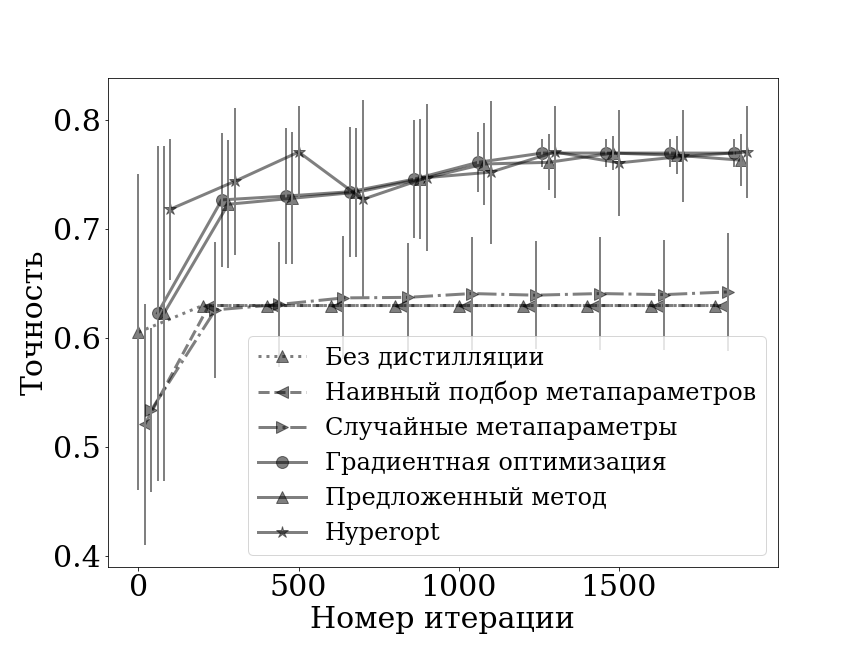
\includegraphics[width=\linewidth]{ait-utf/synth_accuracy_rus_greyscale.png}\\а)}
    % \caption{}
    \label{fig:epoch_size}
    \end{subfigure}
    \begin{subfigure}[h]{0.5\linewidth}
    \center{
    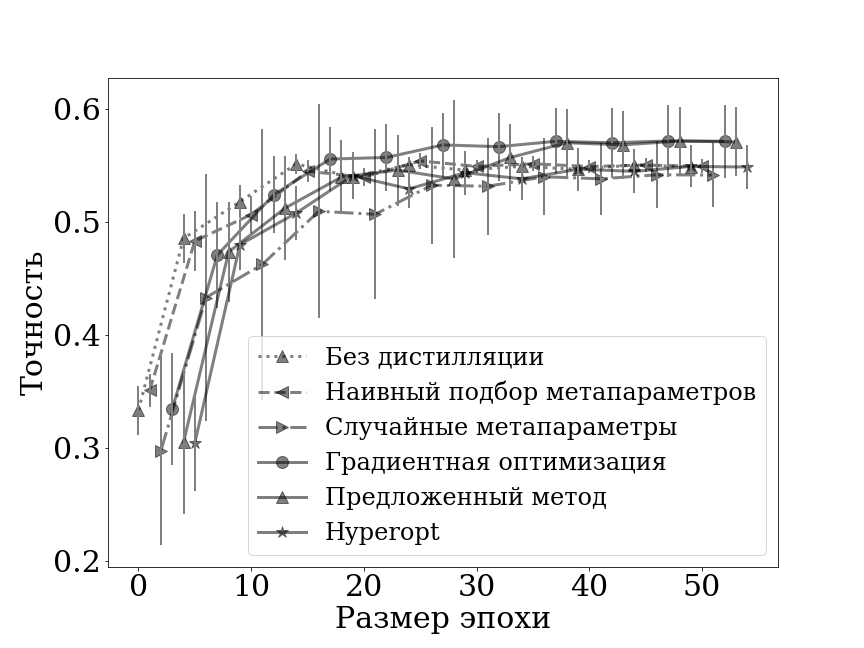
\includegraphics[width=\textwidth]{ait-utf/mini_cifar_accuracy_rus_black.png}\\б)}
    % \caption{}
    \label{fig:train_splines_every_epoch}
    \end{subfigure}
    % \vspace{-0.2 cm}
    \caption{%\fontsize{10}{5}\selectfont
    Точность модели на выборках: a) синтетической, б) уменьшенной CIFAR-10. Здесь и далее точки незначительно смещены относительно оси абсцисс для лучшей читаемости графиков.}
    \label{fig:accuracy}
\end{figure}
 
 
\subsection{Эксперимент на синтетической выборке}
Для оценки полученного метода был проведен эксперимент на синтетической выборке:
\begin{gather*}
    \mathfrak{D} = \{(\mathbf{x}_i, y_i)\}_{i=1}^{m}, \quad x_{ij} \in \mathcal{N}(0, 1),\; j=1, 2, \quad x_{i3} = [\text{sign}(x_{i1})+\text{sign}(x_{i2})>0],\\
    y_i = \text{sign}(x_{i1}\cdot x_{i2}+\delta),
\end{gather*}
где~$\delta \in \mathcal{N}(0, 0.5)$ --- это шум. Размер выборки модели-ученика значительно меньше размера выборки модели-учителя и  $\mathfrak{D}_\text{train}$. Для корректной демонстрации предложенного метода в этом эксперименте выборка была поделена на 3 части: обучающая выборка для модели-учителя, состоящая из 200 объектов, обучающая выборка для модели-ученика, состоящая из 15 объектов, и валидационная выборка, которая также является тестовой, $\mathfrak{D}_\text{val} = \mathfrak{D}_\text{test}$. Она также состоит из 200 объектов. Визуализация выборки изображена на Рис.~\ref{fig:synth}. Модель-учитель была обучена на протяжении 20000 итераций методом стохастического градиентного спуска с длиной шага, равной $10^{-2}.$ Для ее обучения было использовано модифицированное признаковое пространство:
\[
    x_{i3} = [\text{sign}(x_{i1})+\text{sign}(x_{i2}) + 0.1 >0].
\]

Данная модификация не позволяет модели-учителю безошибочно предсказывать обучающую выборку. В данном случае, для обучения модели-ученика предпочтительно использование только слагаемого дистилляции, $\lambda_1 = 0$. Обучение модели-ученика происходило на протяжении 2000 итераций методом стохастического градиентного спуска с длиной шага, равной 1.0 и $T_\text{val} = 0.1.$

Была проведена серия экспериментов для определения наилучших значений $e_1$ и $e_2$. На Рис. \ref{fig:epoch_size}.а приведен график точности для различных $e_1$ с $e_2$ равным 10. На Рис. \ref{fig:epoch_size}.б изображена точность для различных значений $e_2$. Можно заметить, что с возрастанием $e_1$ и $e_2$ качество аппроксимации траектории обновления метапараметров уменьшается.

\begin{figure}[ht]
    % \fontsize{5}{5}\selectfont
    \begin{subfigure}[h]{0.325\linewidth}
    \center{
    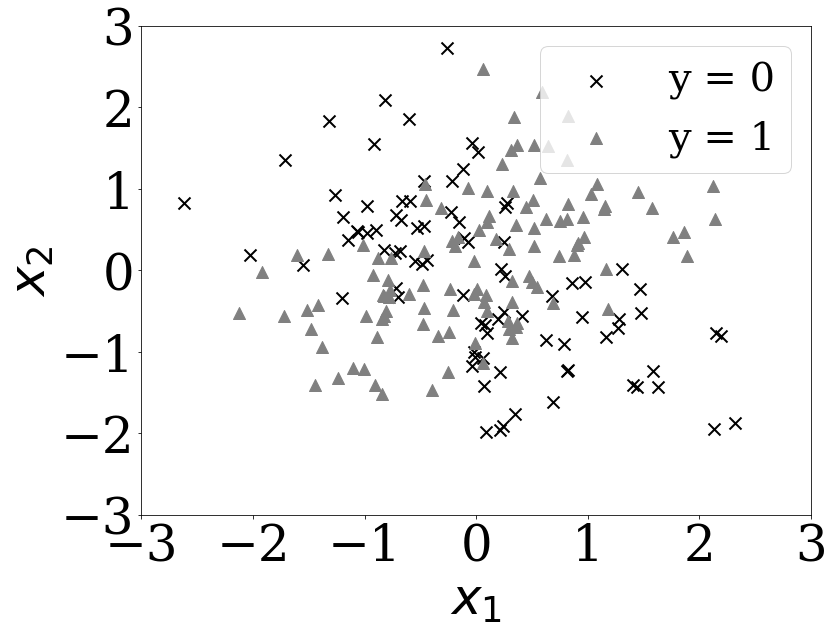
\includegraphics[width=\linewidth]{ttrain_greyscale.png}
    %\caption{}
    \\а)}
    \end{subfigure}
    % \hspace{-0.2cm}
    \begin{subfigure}[h]{0.325\linewidth}
    \center{
    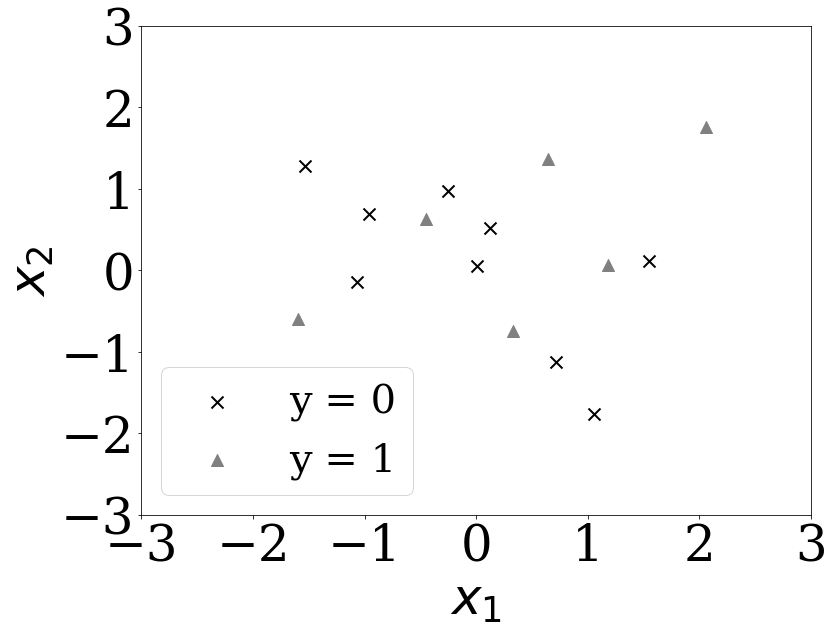
\includegraphics[width=\linewidth]{train_greyscale.png}
    %\caption{}
    \\б)}
    \end{subfigure}
    \begin{subfigure}[h]{0.325\linewidth}
    \center{
    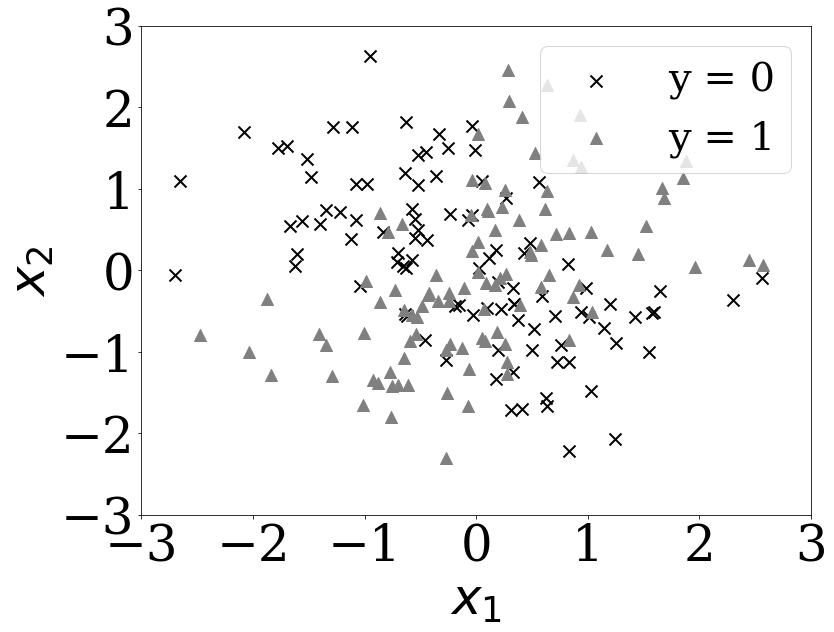
\includegraphics[width=\linewidth]{test_greyscale.png}
    %\caption{}
    \\в)}
    \end{subfigure}
    
    % \vspace{-0.2 cm}
    
    \caption{%\fontsize{8}{5}\selectfont
    Визуализация выборки для а) модели-учителя; б) модели-ученика; в) тестовой выборки}
    \label{fig:synth}
\end{figure}


\begin{figure}[ht]
    \begin{subfigure}[h]{0.5\linewidth}
    \center{
    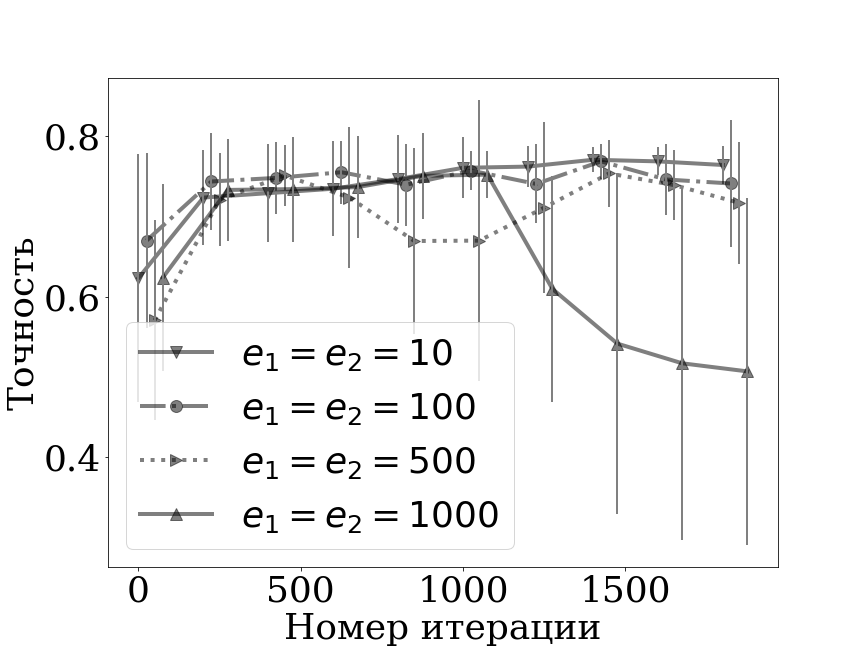
\includegraphics[width=\linewidth]{ait-utf/synth_mini_epoch_size_rus_greyscale.png}\\а)}
    % \caption{}
    \label{fig:epoch_size}
    \end{subfigure}
    \begin{subfigure}[h]{0.5\linewidth}
    \center{
    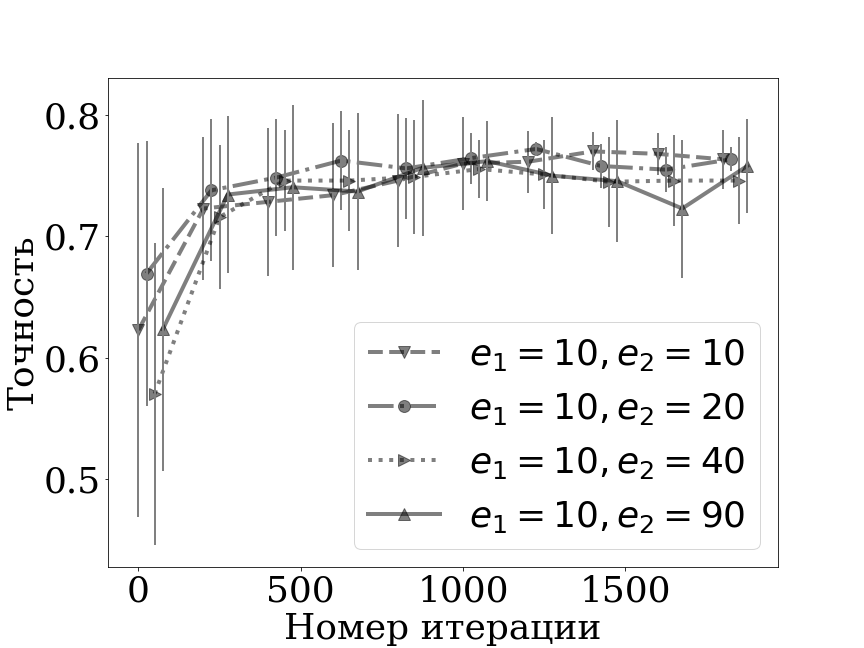
\includegraphics[width=\linewidth]{ait-utf/synth_period_rus_greyscale.png}
    \\б)}
    % \caption{}
    \label{fig:train_splines_every_epoch}
    \end{subfigure}
    % \vspace{-0.2 cm}
    \caption{%\fontsize{10}{5}\selectfont
    Точность модели со значениями $e_1$ и $e_2$: а) $e_1 = e_2$; б) подбор $e_2$ при $e_1 = 10$.}
    \label{fig:epoch_size}
\end{figure}
 

На рис. \ref{fig:accuracy}.a изображена точность модели для различных методов. Наилучшие результаты были получены для оптимизированных значений метапараметров и предложенного метода. Можно заметить, что предложенный метод хорошо аппроксимирует оптимизацию метапараметров в данном эксперименте.

\subsection{Эксперименты на выборках CIFAR-10 и Fashion-MNIST}

Обе выборки были разделены в пропорции 9:1 для обучения и валидации. Для оптимизации параметров модели был использован метод стохастического градиентного спуска с начальной длиной шага, равной 1.0. Длина шага умножалась на 0.5 каждые 10 эпох. Значение $T_\text{val}$ задано равным 1.0.

Для эксперимента на выборке CIFAR-10 была использована предобученная модель ResNet из~\cite{pkt_eccv} в качестве модели-учителя. В качестве модели-ученика была использована модель CNN с тремя сверточными слоями и двумя полносвязными слоями.

Для экспериментов на уменьшенной выборке длина шага для оптимизации метапараметров была равна 0.25 и модель обучалась 50 эпох. Для эксперимента на полной выборке была использована дина шага, равная 0.1. Модель обучалась 100 эпох. 

Для эксперимента на выборке Fashion-MNIST использовались архитектуры модели-ученика и модели-учителя, аналогичные архитектурам в эксперименте на выборке CIFAR-10. Для оптимизации метапараметров была использована длина шага, равная 0.1 и модель обучалась 50 эпох.

Из результатов в Таблице~\ref{table:results} видно, что предложенный метод и градиентные методы дают высокое значение точности. Однако, недостаток  градиентных методов заключается в <<застревании>> в точках локального минимума, из-за чего дисперсия результатов получается гораздо выше, чем у остальных методов. Этот эффект можно заметить на Рис.~\ref{fig:accuracy} и в Таблице~\ref{table:results}.


\section{Заключение}

Была исследована задача оптимизации параметров модели глубокого обучения. Было предложено обобщение методов дистилляции, заключающееся в градиентной оптимизации метапараметров. На первом уровне оптимизируются параметры модели, на втором --- метапараметры, задающие вид оптимизационной задачи. Был предложен метод, уменьшающий вычислительную сложность оптимизации метапараметров для градиентной оптимизации.   Были исследованы свойства оптимизационной задачи и методы предсказания траектории оптимизации метапараметров модели. Под метапараметрами модели понимаются параметры оптимизационной задачи дистилляции. Предложенное обобщение позволило производить дистилляцию модели с лучшими эксплуатационными характеристиками и за меньшее число итераций оптимизации.  Данный подход был проиллюстрирован с помощью вычислительного эксперимента на выборках CIFAR-10 и Fashion-MNIST, и на синтетической выборке. Вычислительный эксперимент показал эффективность градиентной оптимизации для задачи выбора метарапараметров функции потерь дистилляции. Проанализирована возможность аппроксимировать траекторию оптимизации метапараметров локально-линейной моделью. Планируется дальнейшее исследование оптимизационной задачи и анализ качества аппроксимации траектории оптимизации метапараметров более сложными прогностическими моделями.


\begin{thebibliography}{10}

\bibitem{journals/anor/BakhteevS20}
{\it Bakhteev O.Y., Strijov V.V.}
Comprehensive analysis of gradient-based hyperparameter optimization algorithms // Ann. Oper. Res, 2020. Vol. 289. No. 1. P. 51--65.

\bibitem{bergstra2012random}
{\it Bergstra J., Bengio Y.}
Random search for hyper-parameter optimization. // Journal of machine learning research, 2012. Vol. 13. No. 2.

\bibitem{bergstra2013making}
{\it Bergstra J., Yamins D., Cox D.}
Making a science of model search:  Hyperparameter optimization in hundreds of dimensions for vision architectures // International conference on machine learning. -- 2013. P. 115--123.

\bibitem{bishop2006pattern}
{\it Bishop C.M.}
Pattern recognition and machine learning (information science and statistics). -- 2006.

\bibitem{journals/corr/HintonVD15}
{\it Hinton G.E., Vinyals O., Dean J.}
Distilling the knowledge in a neural network // CoRR, 2015. Vol. abs/1503.02531. URL: http://arxiv.org/abs/1503.02531.

\bibitem{krizhevsky2009learning}
{\it Krizhevsky A., et al.}
Learning multiple layers of features from tiny images, 2009.

\bibitem{liu2018darts}
{\it Liu H., Simonyan K., Yang Y.}
Darts:  Differentiable architecture search // arXiv preprint arXiv:1806.09055, 2018.

\bibitem{journals/corr/LuketinaBR15}
{\it Luketina J., Berglund M., Greff K., Raiko T.}
Scalable gradient-based tuning of continuous regularization hyperparameters // CoRR, 2015. Vol. abs/1511.06727. URL: http://arxiv.org/abs/1511.06727.

\bibitem{journals/corr/MaclaurinDA15}
{\it Maclaurin D., Duvenaud D., Adams R.P.}
Gradient-based hyperparameter optimization through reversible learning // CoRR, 2015. Vol. abs/1502.03492. URL: http://arxiv.org/abs/1502.03492.

\bibitem{conf/cvpr/PassalisTT20}
{\it Passalis N., Tzelepi M., Tefas A.}
Heterogeneous knowledge distillation using information flow modeling // CVPR. -- 2020.  P. 2336--2345. URL: https://ieeexplore.ieee.org/xpl/conhome/9142308/proceeding.

\bibitem{pkt_eccv}
{\it Passalis N., Tzelepi M., Tefas A.}
Heterogeneous knowledge distillation using information flow modeling // Proceedings of the IEEE Conference on Computer Vision and Pattern Recognition. -- 2020.

\bibitem{journals/corr/Pedregosa16}
{\it Pedregosa F.}
Hyperparameter optimization with approximate gradient // CoRR, 2016. Vol. abs/1602.02355. URL: http://arxiv.org/abs/1602.02355.

\bibitem{rasley2020deepspeed}
{\it Rasley J., Rajbhandari S., Ruwase O., He Y.}
Deepspeed: System optimizations enable training deep learning models with over 100 billion parameters // Proceedings of the 26th ACM SIGKDD International Conference on Knowledge Discovery \& Data Mining. -- 2020. P. 3505--3506.

\bibitem{Vatanen}
{\it Vatanen T. et al.}
Pushing stochastic gradient towards second-order methods – backpropagation learning with transformations in nonlinearities // International Conference on Neural Information Processing. – Springer, Berlin, Heidelberg, 2013. – P. 442–449.

\bibitem{journals/corr/abs-1708-07747}
{\it Xiao H., Rasul K., Vollgraf R.}
Fashion-mnist: a novel image dataset for benchmarking machine learning algorithms // CoRR, 2017. Vol. abs/1708.07747. URL: http://arxiv.org/278abs/1708.07747.


\bibitem{source_code}
Код вычислительного эксперимента. 
URL: https://github.com/Intelligent-Systems-Phystech/2021-Project-84. Дата обращения: 30.01.2022.

\end{thebibliography}


\AdditionalInformation{Горпинич М.}{Московский физико-технический институт (государственный университет), студент, Долгопрудный}{gorpinich4@gmail.com}

\AdditionalInformation{Бахтеев О.Ю.}{Вычислительный центр имени А.А. Дородницына Федерального исследовательского центра
«Информатика и управление» Российской академии наук, к.ф.-м.н., Москва}{bakhteev@phystech.edu}

\AdditionalInformation{Стрижов В.В.}{Вычислительный центр имени А.А. Дородницына Федерального исследовательского центра
«Информатика и управление» Российской академии наук, д.ф.-м.н., Москва}{strijov@ccas.ru}


\end{document}
